\newcommand{\CLASSINPUTtoptextmargin}{2.5cm}
\newcommand{\CLASSINPUTbottomtextmargin}{2cm}
\documentclass[a4paper, 11pt, oneside]{article}
\usepackage{url}
\usepackage[T1]{fontenc}
\usepackage[utf8]{inputenc}
\usepackage{xcolor}
\usepackage{amsmath}
\usepackage{amssymb}
%\usepackage{cmbright}
\usepackage{algorithm}
\usepackage{algorithmic}
\usepackage{sansmathfonts}
\usepackage{wrapfig}


\newcommand{\red}[1]{\begin{color}{red}#1\end{color}}

%\usepackage{geometry}
%\geometry{letterpaper, margin=1.3in}

\usepackage[acronyms,nonumberlist,nopostdot,nomain,nogroupskip]{glossaries}
\usepackage{tablefootnote}
%\usepackage{booktabs}
\usepackage{tabularx}
\usepackage{tikz}
\usepackage{pgfplots}
\pgfplotsset{compat=newest}
\pgfplotsset{plot coordinates/math parser=false}
\newlength\fheight
\newlength\fwidth
\usetikzlibrary{plotmarks,patterns,decorations.pathreplacing,backgrounds,calc,arrows,arrows.meta,spy,matrix}
\usepgfplotslibrary{patchplots,groupplots}
\usepackage{tikzscale}

\usepackage{multirow}
\usepackage{tkz-kiviat}

\renewcommand{\figurename}{Figure}
%\renewcommand{\tablename}{Tab.}


\usepackage{mathtools}
\usepackage[affil-it]{authblk}
\renewcommand{\abstractname}{Summary}
\renewcommand{\algorithmicrequire}{\textbf{Input:}}
\renewcommand{\algorithmicensure}{\textbf{Output:}}

\usepackage[font=small]{subcaption}
\usepackage[font=small]{caption}
\usepackage{hyperref}

\newcommand{\MP}[1]{\color{red}{\textbf{MP says: #1 }}\color{black}}

\usepackage{dblfloatfix}    % To enable figures at the bottom of page
\usepackage{colortbl}

\newacronym{3gpp}{3GPP}{3rd Generation Partnership Project}
\newacronym{adc}{ADC}{Analog to Digital Converter}
\newacronym{afbw}{AFBW}{Average Fading Bandwidth}
\newacronym{5g}{5G}{5th generation}
\newacronym{aimd}{AIMD}{Additive Increase Multiplicative Decrease}
\newacronym{am}{AM}{Acknowledged Mode}
\newacronym{amc}{AMC}{Adaptive Modulation and Coding}
\newacronym{aqm}{AQM}{Active Queue Management}
\newacronym{awgn}{AGWN}{Additive White Gaussian Noise}
\newacronym{balia}{BALIA}{Balanced Link Adaptation}
\newacronym{bsr}{BSR}{Buffer Status Report}
\newacronym{bdp}{BDP}{Bandwidth-Delay Product}
\newacronym{bf}{BF}{Beamforming}
\newacronym{isp}{ISP}{Internet Service Provider}
\newacronym{ngnm}{NGNM}{Next Generation Mobile Networks Alliance}
\newacronym{cc}{CC}{Component Carrier}
\newacronym{drb}{DRB}{Data Radio Bearer}
\newacronym{qos}{QoS}{Quality of Service}
\newacronym{ca}{CA}{Carrier Aggregation}
\newacronym{lc}{LC}{Logical Channel}
\newacronym{rnti}{RNTI}{Radio Network Temporary Identifier}
\newacronym{qci}{QCI}{Quality Class Identifier}
\newacronym{cdf}{CDF}{Cumulative Distribution Function}
\newacronym{cn}{CN}{Core Network}
\newacronym{cqi}{CQI}{Channel Quality Information}
\newacronym{cir}{CIR}{Channel Impulse Response}
\newacronym{cp}{CP}{Control Plane}
\newacronym{csirs}{CSI-RS}{Channel State Information - Reference Signal}
\newacronym{dc}{DC}{Dual Connectivity}
\newacronym{dce}{DCE}{Direct Code Execution}
\newacronym{dci}{DCI}{Downlink Control Information}
\newacronym{dl}{DL}{Downlink}
\newacronym{dmr}{DMR}{Deadline Miss Ratio}
\newacronym{dmrs}{DMRS}{DeModulation Reference Signal}
\newacronym{e2e}{E2E}{End-to-End}
\newacronym{ecn}{ECN}{Explicit Congestion Notification}
\newacronym{edf}{EDF}{Earliest Deadline First}
\newacronym{enb}{eNB}{evolved Node Base}
\newacronym{embb}{eMBB}{enhanced Mobile Broadband}
\newacronym{epc}{EPC}{Evolved Packet Core}
\newacronym{es}{ES}{Edge Server}
\newacronym{fdma}{FDMA}{Frequency Division Multiple Access}
\newacronym{fdd}{FDD}{Frequency Division Duplexing}
\newacronym[firstplural=Radio Access Technologies (RATs)]{rat}{RAT}{Radio Access Technology}
\newacronym{fs}{FS}{Fast Switching}
\newacronym{ftp}{FTP}{File Transfer Protocol}
\newacronym{gnb}{gNB}{Next Generation Node Base}
\newacronym{harq}{HARQ}{Hybrid Automatic Repeat reQuest}
\newacronym{hetnet}{HetNet}{Heterogeneous Network}
\newacronym{hh}{HH}{Hard Handover}
\newacronym{hol}{HOL}{Head-of-Line}
\newacronym{ia}{IA}{Initial Access}
\newacronym{imt}{IMT}{International Mobile Telecommunication}
\newacronym{iot}{IoT}{Internet of Things}
\newacronym{lcr}{LCR}{Level Crossing Rate}
\newacronym{lcf}{LCF}{Level Crossing Frequency}
\newacronym{los}{LoS}{Line-of-Sight}
\newacronym{lte}{LTE}{Long Term Evolution}
\newacronym{m2m}{M2M}{Machine to Machine}
\newacronym{mac}{MAC}{Medium Access Control}
\newacronym{mc}{MC}{Multi-Connectivity}
\newacronym{mcs}{MCS}{Modulation and Coding Scheme}
\newacronym{mec}{MEC}{Mobile Edge Cloud}
\newacronym{mi}{MI}{Mutual Information}
\newacronym{mimo}{MIMO}{Multiple Input, Multiple Output}
\newacronym{mmwave}{mmWave}{millimeter wave}
\newacronym{mptcp}{MPTCP}{Multipath TCP}
\newacronym{mr}{MR}{Maximum Rate}
\newacronym{mss}{MSS}{Maximum Segment Size}
\newacronym{mtd}{MTD}{Machine-Type Device}
\newacronym{mtu}{MTU}{Maximum Transmission Unit}
\newacronym{nfv}{NFV}{Network Function Virtualization}
\newacronym{nlos}{NLoS}{Non-Line-of-Sight}
\newacronym{nr}{NR}{New Radio}
\newacronym{o2i}{O2I}{Outdoor-to-Indoor}
\newacronym{ofdm}{OFDM}{Orthogonal Frequency Division Multiplexing}
\newacronym{pdcch}{PDCCH}{Physical Downlonk Control Channel}
\newacronym{pdcp}{PDCP}{Packet Data Convergence Protocol}
\newacronym{pdsch}{PDSCH}{Physical Downlink Shared Channel}
\newacronym{pdu}{PDU}{Packet Data Unit}
\newacronym{pf}{PF}{Proportional Fair}
\newacronym{pgw}{PGW}{Packet Gateway}
\newacronym{phy}{PHY}{Physical}
\newacronym{pbch}{PBCH}{Physical Broadcast Channel}
\newacronym[plural=\gls{mme}s,firstplural=Mobility Management Entities (MMEs)]{mme}{MME}{Mobility Management Entity}
\newacronym{prb}{PRB}{Physical Resource Block}
\newacronym{pss}{PSS}{Primary Synchronization Signal}
\newacronym{pucch}{PUCCH}{Physical Uplink Control Channel}
\newacronym{pusch}{PUSCH}{Physical Uplink Shared Channel}
\newacronym{rach}{RACH}{Random Access Channel}
\newacronym{ran}{RAN}{Radio Access Network}
\newacronym{red}{RED}{Random Early Detection}
\newacronym{rf}{RF}{Radio Frequency}
\newacronym{rlc}{RLC}{Radio Link Control}
\newacronym{rlf}{RLF}{Radio Link Failure}
\newacronym{rrc}{RRC}{Radio Resource Control}
\newacronym{rrm}{RRM}{Radio Resource Management}
\newacronym{rr}{RR}{Round Robin}
\newacronym{rs}{RS}{Remote Server}
\newacronym{rsrp}{RSRP}{Reference Signal Received Power}
\newacronym{rss}{RSS}{Received Signal Strength}
\newacronym{rtt}{RTT}{Round Trip Time}
\newacronym{rw}{RW}{Receive Window}
\newacronym{rx}{RX}{Receiver}
\newacronym{sa}{SA}{standalone}
\newacronym{sack}{SACK}{Selective Acknowledgment}
\newacronym{sap}{SAP}{Service Access Point}
\newacronym{sch}{SCH}{Secondary Cell Handover}
\newacronym{scoot}{SCOOT}{Split Cycle Offset Optimization Technique}
\newacronym{sdma}{SDMA}{Spatial Division Multiple Access}
\newacronym{sinr}{SINR}{Signal-to-Interference-plus-Noise Ratio}
\newacronym{sir}{SIR}{Signal-to-Interference Ratio}
\newacronym{sm}{SM}{Saturation Mode}
\newacronym{snr}{SNR}{Signal-to-Noise Ratio}
\newacronym{son}{SON}{Self-Organizing Network}
\newacronym{ss}{SS}{Synchronization Signal}
\newacronym{srs}{SRS}{Sounding Reference Signal}
\newacronym{sss}{SSS}{Secondary Synchronization Signal}
\newacronym{tb}{TB}{Transport Block}
\newacronym{tcp}{TCP}{Transmission Control Protocol}
\newacronym{tdd}{TDD}{Time Division Duplexing}
\newacronym{tdma}{TDMA}{Time Division Multiple Access}
\newacronym{tfl}{TfL}{Transport for London}
\newacronym{tm}{TM}{Transparent Mode}
\newacronym{trp}{TRP}{Transmitter Receiver Pair}
\newacronym{tti}{TTI}{Transmission Time Interval}
\newacronym{ttt}{TTT}{Time-to-Trigger}
\newacronym{tx}{TX}{Transmitter}
\newacronym{ue}{UE}{User Equipment}
\newacronym{ul}{UL}{Uplink}
\newacronym{uml}{UML}{Unified Modeling Language}
\newacronym{um}{UM}{Unacknowledged Mode}
\newacronym{uma}{UMa}{Urban Macro}
\newacronym{utc}{UTC}{Urban Traffic Control}
\newacronym{vm}{VM}{Virtual Machine}
\newacronym{rsrq}{RSRQ}{Reference Signal Received Quality}
\newacronym{rssi}{RSSI}{Received Signal Strength Indicator}
\newacronym{crs}{CRS}{Cell Reference Signal}
\newacronym{nsa}{NSA}{Non Stand Alone}
\newacronym{mrdc}{MR-DC}{Multi \gls{rat} \gls{dc}}
\newacronym{endc}{EN-DC}{E-UTRAN-\gls{nr} \gls{dc}}
\newacronym{5gc}{5GC}{5G Core}
\newacronym{si}{SI}{Study Item}
\newacronym{iab}{IAB}{Integrated Access and Backhaul}
\newacronym{wf}{WF}{Wired-first}
\newacronym{hqf}{HQF}{Highest-quality-first}
\newacronym{pa}{PA}{Position-aware}
\newacronym{mlr}{MLR}{Maximum-local-rate}
\newacronym{wbf}{WBF}{Wired Bias Function}
\newacronym{mib}{MIB}{Master Information Block}
\newacronym{sib}{SIB}{Secondary Information Block}
\newacronym{kpi}{KPI}{Key Performance Indicator}
\newacronym{ppp}{PPP}{Poisson Point Process}
\newacronym{mpc}{MPC}{Multi Path Component}
\newacronym{rt}{RT}{Ray Tracer}
\newacronym{aoa}{AoA}{Angle of Arrival}
\newacronym{aod}{AoD}{Angle of Departure}
\newacronym{scm}{SCM}{Spatial Channel Model}
\newacronym{inr}{INR}{Interference to Noise Ratio}
\newacronym{qd}{QD}{Quasi Deterministic}
\newacronym{wlan}{WLAN}{Wireless Local Area Network}
\newacronym{cad}{CAD}{Computer-aided Design}
\newacronym{ap}{AP}{Access Point}
\newacronym{sta}{STA}{Station}
\newacronym{urllc}{URLLC}{Ultra-Reliable Low-Latency Communication}
\newacronym{udp}{UDP}{User Datagram Protocol}
\newacronym{laa}{LAA}{Licensed-Assisted Access}
% tikz styles
\tikzstyle{startstop} = [rectangle, rounded corners, minimum width=2cm, minimum height=0.5cm,text centered, draw=black]
\tikzstyle{io} = [trapezium, trapezium left angle=70, trapezium right angle=110, minimum width=3cm, minimum height=1cm, text centered, draw=black]
\tikzstyle{process} = [rectangle, minimum width=2cm, minimum height=0.5cm, text centered, draw=black, alignb=center]
\tikzstyle{decision} = [ellipse, minimum width=2cm, minimum height=1cm, text centered, draw=black]
\tikzstyle{arrow} = [thick,<->,>=stealth]
\tikzstyle{line} = [thick,>=stealth]
\tikzstyle{darrow} = [thick,<->,>=stealth,dashed]
\tikzstyle{sarrow} = [thick,->,>=stealth]
%\tikzstyle{larrow} = [line width=0.05mm,dashdotted,>=stealth]
\tikzstyle{larrow} = [line width=0.1mm,dashdotted,->,>=stealth]


\makeatletter
\def\grd@save@target#1{%
  \def\grd@target{#1}}
\def\grd@save@start#1{%
  \def\grd@start{#1}}
\tikzset{
  grid with coordinates/.style={
    to path={%
      \pgfextra{%
        \edef\grd@@target{(\tikztotarget)}%
        \tikz@scan@one@point\grd@save@target\grd@@target\relax
        \edef\grd@@start{(\tikztostart)}%
        \tikz@scan@one@point\grd@save@start\grd@@start\relax
        \draw[minor help lines] (\tikztostart) grid (\tikztotarget);
        \draw[major help lines] (\tikztostart) grid (\tikztotarget);
        \grd@start
        \pgfmathsetmacro{\grd@xa}{\the\pgf@x/1cm}
        \pgfmathsetmacro{\grd@ya}{\the\pgf@y/1cm}
        \grd@target
        \pgfmathsetmacro{\grd@xb}{\the\pgf@x/1cm}
        \pgfmathsetmacro{\grd@yb}{\the\pgf@y/1cm}
        \pgfmathsetmacro{\grd@xc}{\grd@xa + \pgfkeysvalueof{/tikz/grid with coordinates/major step x}}
        \pgfmathsetmacro{\grd@yc}{\grd@ya + \pgfkeysvalueof{/tikz/grid with coordinates/major step y}}
        \foreach \x in {\grd@xa,\grd@xc,...,\grd@xb}
        \node[anchor=north] at (\x,\grd@ya) {\pgfmathprintnumber{\x}};
        \foreach \y in {\grd@ya,\grd@yc,...,\grd@yb}
        \node[anchor=east] at (\grd@xa,\y) {\pgfmathprintnumber{\y}};
      }
    }
  },
  minor help lines/.style={
    help lines,
    gray,
    line cap =round,
    xstep=\pgfkeysvalueof{/tikz/grid with coordinates/minor step x},
    ystep=\pgfkeysvalueof{/tikz/grid with coordinates/minor step y}
  },
  major help lines/.style={
    help lines,
    line cap =round,
    line width=\pgfkeysvalueof{/tikz/grid with coordinates/major line width},
    xstep=\pgfkeysvalueof{/tikz/grid with coordinates/major step x},
    ystep=\pgfkeysvalueof{/tikz/grid with coordinates/major step y}
  },
  grid with coordinates/.cd,
  minor step x/.initial=.5,
  minor step y/.initial=.2,
  major step x/.initial=1,
  major step y/.initial=1,
  major line width/.initial=1pt,
}
\makeatother

\def\si{\tikz\fill[scale=0.4](0,.35) -- (.25,0) -- (1,.7) -- (.25,.15) -- cycle;}
\usepackage[a4paper, total={6.2in, 9.2in}]{geometry}
\date{}

\makeglossaries

\begin{document}


\title{\vspace{-1.0cm}\huge \textbf{A hierarchical SIFT matching \\ implementation in C\texttt{++}} }
\author[1]{\Large Matteo Pagin}
\affil[1]{Department of Information Engineering, University of Padova}

\maketitle

% 3GPP does not want us to use New Radio, so we disable the expansion of the acronym
\glsunset{nr}
\thispagestyle{empty}

\begin{abstract}
	In recent years the usage of binary-valued features such as BRIEF and ORB has experienced a dramatic upsurge, driven by the following advantages over vector-based solutions: faster computation, quicker comparison and a significantly smaller memory footprint. Nevertheless, these binaries features, especially in certain scenarios, lack the descriptive capability of vector-based features such as SIFT, which in this regard are still capable to outperform solutions like BRIEF and ORB. Therefore, the research efforts have been focusing on combining the strengths of these two approaches. In this regard, a fast SIFT matching algorithm is hereby presented and implemented, featuring the binary quantization of SIFT features in conjunction of a hierarchical-based binary matching technique.
  % In this paper, we propose to perform slicing using carrier aggregation, and introduce RoGeR, a cross-carrier scheduling policy
\end{abstract}

\section*{Introduction}
  The task of detecting salient points and computing their description as features has always been of primary importance in computer vision. This problem has been tackled using primarily two approaches, namely binary descriptors such as BRIEF~\cite{calonder2010brief}, ORB~\cite{rublee2011orb} and vector-based solutions like SIFT~\cite{lowe2004distinctive}. While the former category of descriptors is fast to compute and has a very limited memory footprint, the latter exhibit a top of the class robustness wrt scale and rotation changes, on top of unmatched discriminative capabilities over large datasets~\cite{grauman2005efficient, karami2017image}. It follows that transforming vector features into binary ones apparently promises to offer the best of both worlds; this work is in fact based on the same premise. In particular, the presented implementation leverages a median quantization strategy, which manages to obtain satisfying accuracy while exhibiting low computational complexity~\cite{peker2011binary}.
  
  
  In turn, matching such descriptors has also been another key problem and in such regard the focus of features matching algorithms has also changed over the years: since the size of the available datasets is growing at a staggering pace, the current challenge is to find significant matches in contexts where an exhaustive, linear search is unfeasible. Even though the majority of algorithms sharing such target are based on an approximate nearest neighbour strategy and/or hashing techniques, one of the most promising algorithms for computer vision applications relies on a hierarchical decomposition of the search space~\cite{muja2012fast}.
  
  
  The purpose of this work is to analyze the performance of the combination of the aforementioned approaches, namely the hierarchical-based matching of median-quantized SIFT features.
  \section*{Median quantization}
  A SIFT feature is basically an histogram of gradient directions that is encoded as a $128$-dimensional vector. Since its components take values in the range $[0, 255]$ it follows that SIFT vectors live in a space of $256^{128}$ possible points. In practice though only a small portion of this huge space is actually used: by examining the marginal distributions of the single components it is possible to notice an exponential-like distribution~\cite{peker2011binary}, a phenomenon that indicates that these descriptors do not actually fully exploit their theoretically available expressive power. This is demonstrated even further by the fact that pairwise distances are also relatively small compared to the values that can be expected of in such high dimensional space. It follows that it should be possible to compress the information contained in a SIFT descriptor into a smaller vector, in fact even down to the binary case. In this regard, since the primary goal of this quantization is to preserve the pairwise distances, namely to map similar features vectors into similar binary representations, the optimal strategy is to choose as quantization threshold the median value of a given vector`s components. This choice maximizes the entropy of the quantized feature and it has been empirically shown that it also preserves the pairwise distances, leading to matches that are consistent with the original features representation~\cite{peker2011binary}.
  
  
    \section*{Fast matching of binary features}
Once the SIFT features have been quantized into binary vectors, the presented implementation searches similar descriptors by using the fast matching technique for binary features introduced in~\cite{muja2012fast}. This algorithm essentially decomposes the search space by first building a tree whose non-leaf nodes represent cluster centers and leaf ones contain disjoint subsets of the original features set. Finally this hierarchical structure is used in order to look for matches by performing a number of comparisons that is significantly smaller compared to the linear, exhaustive search case. Clearly this algorithm can be decomposed into two phases: the computation of the hierarchical structures and the subsequent, actual search; the aim is to optimize the complexity of the latter, as the former can be sensibly considered a pre-computation.

\begin{algorithm}[h!]
\begin{algorithmic}[1]
 \REQUIRE Dataset of features $D$, branching factor $K$ and max leaf set size $S_{L}$
 \ENSURE Hierarchical clustering tree
 \IF{$\Vert D \Vert < S_L$} 
 \STATE {create leaf node set with the points of $D$} 
 \ELSE 
 \STATE{$P \leftarrow K$ points selected randomly from $D$}
 \STATE {$C \leftarrow$ list of cluster obtained by partitioning $D$ around the points of $P$} 
 \FOR{each cluster $C_i \in C$} 
 \STATE {create non-leaf node storing the $i$th center} 
 \STATE {recursively apply the algorithm to the points in $C_i$} 
 \ENDFOR
 \ENDIF
 \end{algorithmic}
 \caption{Creation of a hierarchical clustering tree}\label{Alg:treec}
\end{algorithm}

The creation of the tree is performed by recursively clustering the original set into a pre-determined amount of clusters $K$: first of all $K$ points of the dataset are randomly chosen as centers and stored in non-leaf nodes of the tree, then the set points are partitioned around such centers and are placed as their children. Such process it then repeated in a recursive manner until the cluster size is smaller than a given threshold, as can be seen in Alg.~\ref{Alg:treec}.
 Actually, the algorithm uses multiple copies of such trees; the rationale behind such choice is that since the centers selection is completely random, different trees are likely to have extremely different structures that may lead to quite heterogeneous times needed to reach the target leaf node in the tree. Therefore, by using these structures in parallel the resulting search time is the minimum of such value across all the trees, effectively increasing the chance of finding a match in a small amount of time. 

\begin{minipage}{0.45\textwidth}
\begin{algorithm}[H]
    \centering
    \caption{Parallel search of hierarchical clustering trees}\label{Alg:search}
    \begin{algorithmic}[1]
		\REQUIRE Hierarchical clustering trees $T_i$, query point $Q$, max amount of points to examine $L_{max}$
		\ENSURE $K$ nearest approximate neighbours of $Q$
		\STATE {$L \leftarrow 0$ counter of searched points}
		\STATE {$PQ, R \leftarrow$ empty priority queues}
		\FOR{each tree $T_i$} 
		\STATE {\texttt{TraverseTree$(T_i, PQ, R, Q)$}} 
		\ENDFOR
		\WHILE {$PQ \neq \emptyset$ and $L < L_{max}$} 
		\STATE {$N \leftarrow$ top of $PQ$} 
		\STATE {\texttt{TraverseTree$(N, PQ, R, Q)$}} 
		\ENDWHILE
		\RETURN $K$ points of $R$ that are closer to $Q$
    \end{algorithmic}
\end{algorithm}
\end{minipage}
\hfill
\begin{minipage}{0.45\textwidth}
\begin{algorithm}[H]
    \centering
    \caption{\texttt{TraverseTree$(N, PQ, R, Q)$}}\label{Alg:traverse}
    \begin{algorithmic}[1]
	    \REQUIRE Specific node of a clustering trees $N$, query point $Q$, amount of leaves examined $L$
		\ENSURE Updated main queue $R$ and auxiliary refinement queue $PQ$
		 \IF{$N$ is a leaf node} 
		 \STATE {linearly search all points $\in N$ and add them to $R$} 
		 \STATE{$L \leftarrow L + \Vert N \Vert$ }
		 \ELSE 
		 \STATE{$C \leftarrow$ child nodes of $N$}
		 \STATE{$N' \leftarrow$ closes node of $C$ to $Q$}
		 \STATE {$C_p \leftarrow C \setminus N'$} 
		 \STATE {add the nodes of $C_p$ to $PQ$} 
		 \STATE {\texttt{TraverseTree$(N', PQ, R)$}} 
		 \ENDIF
    \end{algorithmic}
\end{algorithm}
\end{minipage}

\bigskip

The actual process of scanning these hierarchical data structures in order to find significant matches starts by performing a single traverse of the pre-computed trees. During this initial traversal, the node which is the closest to the query is picked and the search continues in a recursive fashion on that very same node until a leaf is reached. Upon such event, the points contained in the leaf are linearly scanned and added to the main queue $R$; on the other hand the nodes that we neglect along the way are progressively added to an auxiliary priority queue $PQ$, as explained in Alg.~\ref{Alg:traverse}. Once the first traverse has been undertaken, a refinement of the search is performed by progressive traversals of the nodes contained in $PQ$, until either we reach the end of the queue or the amount of points visited surpasses the threshold $L_{max}$. The latter process allows to improve the accuracy of the results: in fact $L_{max}$ gives as the possibility to fine-tune the trade-off between precision of the search algorithm and its computational cost, therefore rending the whole procedure flexible and possibly suited to different use-cases. Finally, the max amount of leaves and the branching factor do not have a significant impact on the search performance but they have the potential to sensibly influence the tress build time. Once again, this allows to tune the algorithm to the specific application, as some of them may consider the tree creation as a pre-computation, while others may need to do that in real-time, hence exhibit the need of faster hierarchical structures creation.

    
\begin{figure}[h!]
  \centering
    % this sets the width of the figure, adjust to your needs
    \setlength\fwidth{0.7\columnwidth}
    % this sets the height of the figure, adjust to your needs
    \setlength\fheight{0.2\columnwidth}
    
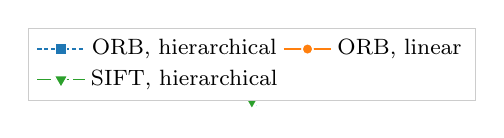
\begin{tikzpicture}
\pgfplotsset{every tick label/.append style={font=\scriptsize}}

\definecolor{color0}{rgb}{0.12156862745098,0.466666666666667,0.705882352941177}
\definecolor{color1}{rgb}{1,0.498039215686275,0.0549019607843137}
\definecolor{color2}{rgb}{0.172549019607843,0.627450980392157,0.172549019607843}

\begin{axis}[
width=\fwidth,
height=\fheight,
at={(0\fwidth,0\fheight)},
scale only axis,
% axis line style={white!80!black},
legend style={at={(0.5,0.95)}, anchor=south, draw=white!80!black, font=\footnotesize},
legend columns=2,
% tick align=outside,
% x grid style={white!80!black},
xlabel style={font=\footnotesize},
xlabel={amount of SIFT features},
xmajorgrids,
% xmajorticks=false,
xmin=1, xmax=210,
xtick style={color=white!15!black},
% y grid style={white!80!black},
ylabel shift = -3 pt,
ylabel style={font=\footnotesize},
ylabel={Normalized Hamming distance cost},
ymajorgrids,
% ymajorticks=false,
ymin=0, ymax=1.1,
ytick style={color=white!15!black},
axis background/.style={fill=white},
ymode=log,
log basis y={10}
]

\addplot [semithick, color0, dash pattern=on 1.5pt off 1pt, mark=square*, mark size=2, mark options={solid,draw=white}]
table {%
50 0.00625
100 0.0125
200 0.0425
};
\addlegendentry{ORB, hierarchical}

\addplot [semithick, color1, mark=*, mark size=2, mark options={solid,draw=white}]
table {%
50 0.0626
100 0.25
200 1
};
\addlegendentry{ORB, linear}

\addplot [semithick, color2, dash pattern=on 5pt off 1.5pt, mark=triangle*, mark size=3, mark options={solid,rotate=180,draw=white}]
table {%
50 0.0057
100 0.0114
200 0.0388
};
\addlegendentry{SIFT, hierarchical}
\end{axis}
\end{tikzpicture}



    \setlength\belowcaptionskip{-.3cm}
    \captionsetup{justification=centering}
    \caption{Normalized computational cost of the search subroutines as the amount of computed features ranges $\in \{50, 100, 200\}$. The Y axis uses a logarithmic scale.}
    \label{Fig:perf_cost}
\end{figure}    

\section*{Implementation details and performance evaluation} 
The implementation that is hereby presented\footnote{Available at: \url{https://github.com/pagmatt/bin-features-matching}} leverages both aforementioned algorithms, specifically it uses median quantization on SIFT features and then finds matches among them by performing the fast matching introduced in~\cite{muja2012fast}. The programming language that has been chosen for the task is C\texttt{++}, due to the performance-oriented nature of these algorithms. On top of the language standard library, the implementation makes use of an open-source, template-based tree library\footnote{\url{https://github.com/kpeeters/tree.hh}} and of OpenCV\footnote{\url{https://github.com/opencv/opencv}} in order to compute the ORB and SIFT features from the dataset images.


In order to carry out the performance evaluation of the presented strategy a linear, exhaustive search among the whole dataset approach has been selected as baseline. Regarding the performance indicators, computational cost and search accuracy have been elected as the two most crucial factors. Furthermore, the complexity of the algorithm has been measured in number of CPU cycles (and their relative load), in order to provide as much abstraction from the underlying hardware as possible. This goal has been met by executing the program via the debugger Valgrind, enabling its profiling tool Callgrind\footnote{\url{https://linux.die.net/man/1/callgrind}} and finally analyzing the output traces in Kcachegrind. An important remark is that during such profiling the tree creation process has been neglected, focusing on the computational cost of the search subroutines only.
\begin{wrapfigure}{r}{0.5\textwidth}
\vspace{-20pt}
  \begin{center}
    \includegraphics[width=0.45\textwidth]{figures/merged.png}
  \end{center}
  \caption{Top $6$ matches returned by ORB (on the left) and SIFT (on the right). In both cases, the leftmost images are the search queries while the rightmost ones are the corresponding matches.}
  \label{Fig:perf_acc}
\end{wrapfigure}
As can be appreciated in Fig.~\ref{Fig:perf_cost}, the implemented strategy manages to significantly outperform the linear search approach: in fact the hierarchical binary search of quantized SIFT features is also marginally faster than the ORB case: with the quantization process each SIFT descriptor is encoded in as little as a $128$ bits vector, while an ORB feature requires from a min of $128$ to a maximum of $512$ bits. Therefore, the pair-wise Hamming distances computation of quantized SIFT features is actually faster than the ORB case, since it involves a smaller amount of bits. 


Finally, the resulting search accuracy can be observed in Fig.~\ref{Fig:perf_acc}, where the top matches for both ORB and SIFT are exhibited. These samples are obtained through a skimming process of the initial matches set which is based on the Nearest Neighbour Distance Ratio (NNDR) criteria introduced in~\cite{lowe2004distinctive}. 
\clearpage
As expected, SIFT features are capable of offering stronger descriptive capabilities and to outperform in such regard the ORB descriptors, providing in the majority of the cases matches that are indeed relevant ones. Furthermore, perhaps surprisingly, such superiority is not lost after the quantization process, suggesting that in such regard the choice of a median threshold in indeed a successful one.

\section*{Conclusions} 
The presented implementation combines a binary quantization technique with an approximate matching algorithm, managing to provide accurate results with a low computational complexity. Therefore, it is well-suited to modern computer vision applications that need to interact with the massive datasets of the current Big Data era.

\bibliographystyle{IEEEtran}
\bibliography{bibl.bib}

\end{document}
